\section{Datenanalyse}
Nach einer erfolgreichen Kompromittierung eines Angreifers muss unabhängig des verwendeten Honeypotsystems eine Datenanalyse stattfinden. Abhängig des eigentlichen Nutzen des Honeypots für das Netzwerk kann eine Netzwerkanalyse mehr oder weniger aufwendig werden. Wird ein Honeypot als Early-Warning System verwendet wird eine aufwendige Datenanalyse nicht nötig sein. Wird er jedoch als Research Honeypot verwendet, oder ein und die selbe Sicherheitslücke wird auf längere Zeit mehrmalig ausgenutzt, so wird eine ordentlich durchgeführte Datenanalyse notwendig. Folgende Merkmale bestimmen ob eine ausführliche Datenanalyse nach einer Kompromittierung durchgeführt werden soll\cite{grimes.2003a}:

\begin{itemize}	
\item Was ist der eigentliche Zweck des Honeypots? (Production oder Research)
\item Was wird versucht zu schützen?
\item Ist jeder Angriff interessant oder nur die die erfolgreich sind?
\item Ist die Angriffsmethode interessant?
\item Soll herausgefunden werden wer der Hacker ist? Welcher Tools, Techniken oder Mechanismen dieser verwendet?
\item Ist nur die Methode des Zugriffs auf den Honeypot interessant oder auch das was der Hacker auf diesen vorhatte?
\end{itemize}

Allgemein sollte bei einer ausführlichen Datenanalyse (wenn z.B. wie im Falle des Projektes ein Research Honeypot verwendet wird) folgende drei Fragen geklärt werden:

\begin{itemize}
\item War der Angriff manuell oder automatisch?
\item Wie fand die initiale Kompromittierung statt?
\item Was macht der Hacker nachdem er sich Zugriff verschafft hat?
\end{itemize}

\noindent Automatisierte Angriffe kommen häufiger vor als manuelle. Manuelle Kompromittierungsversuche sind jedoch um einiges Gefährlicher als automatisierte, da der Angreifer unerwartet seine Strategie ändern, und unberechenbar auf seinem Zielsystem handeln kann. Automatisierte Angriffe nutzen meist bekannte Sicherheitslücken aus, und hoffen dabei bei einer neue Anwendung eine Zero-Day-Attack auszuführen (nutzt Sicherheitslücken aus die die Programmierer bei der erstmaligen Erscheinung eines Programmes noch nicht behoben haben). 
Automatisierte Angriffe sind relativ einfach an folgenden Eigenschaften erkennbar:
\begin{itemize}
\item Schnelle Zugriffsversuche auf verschieden Art und Weise(zeitlich sehr nah beieinander)
\item Ports oder Exploits, die nicht für das eigene System verfügbar sind werden ausprobiert
\item Dieselbe Zugriffsmethode wird in kurzer Zeit mehrmals ausgeführt, ohne das eine Änderung von Parametern stattfindet
\item Das Tippen ist so schnell das kein Mensch dazu fähig wäre 
\end{itemize}

\noindent Im Gengenzug dazu sind manuelle Hacker durch folgende Merkmale erkennbar:

\begin{itemize}
\item Der verwendetet Exploit Code passt zu dem Zielsystem
\item Wesentlich häufiger vorkommende Tippfehler und wiederholende Eingaben
\item Zeitabstände zwischen Eingaben sind ungleichmäßig
\item Versucht häufig vorher Informationen zu sammeln (Ping, Portscan)
\end{itemize}

\noindent \textbf{Initialer Zugriff auf das System}\\
Die meisten Angriffe bestehen aus zwei verschiedenen Phasen. Das Ziel der ersten Phase besteht darin, Zugriff auf das System zu erhalten, das Ziel der zweite um die eigentlichen Absichten zu verfolgen.\\

\noindent \textbf{Nach dem Zugriff}\\
Der meist wichtigere Teil der Datenanalyse ist der Teil der nach der initialen Kompromittierung stattfindet. Das Ziel ist es herauszufinden, was die Absichten des Hackers waren, welche Daten er gesucht hat (z.B. Kreditkartendaten, Werbeinformationen)oder welche Daten er hinterlassen hat. Meist versucht der Hacker den kompromittierten Rechner als Speicherplatz (für z.B. illegale Daten wie DVDs oder Spiele), oder als Teil eines Botnetzes zu verwenden. \\

\noindent Die Möglichkeiten eines Hackers sind vielfältig, deswegen gibt es(je nach Genauigkeit der Analyse) mehr oder weniger aufwendige Analysearten. Diese sind durch die Implementierungsart des Honeypots meist mit eingeschränkt:\\
\newpage
\noindent\textbf{Low-Interactive Honeypots}\\
Bei Low-Interactive Honeypots hält sich die Datenauswertung in Grenzen. Meist bietet sich nur die Möglichkeit, den Netzwerkverkehr, IDS Log-Files und die Honeypot Log-Files zu analysieren. MEHR!\\

\noindent\textbf{High-Interactive Honeypots}\\
\noindent High-Interactive Honeypots bieten eine hohen Informationsgehalt bei der Datenanalyse. Diese ist jedoch im Vergleich zu den anderen Honeypot Implementierungsarten sehr aufwendig. Für eine ausführliche Analyse sind folgende Schritte notwendig\cite{grimes.2003a}:

\begin{enumerate}
\item Den Honeypot aus dem Netz entfernen
\item RAM Speicherinhalte falls möglich sichern
\item Eine Kopie der Festplatte erstellen
\item Netzwerkverkehr, Dateisystem, Schadcode (falls vorhanden), Betriebssystem, Log-Daten analysieren
\item Schlüsse daraus ziehen (Sicherheitslücken erkennen)
\item Sicherheitslücken schließen/Honeypot modifizieren (falls gewünscht)
\item Honeypot neu aufsetzen
\end{enumerate}

\noindent\textbf{Den Honeypot offline nehmen}\\
\noindent Um eine forensische Analyse an einem Honeypot vorzunehmen, muss zunächst sicher gestellt werden, dass sich dieser nicht mehr im Netz befindet. So wird sichergestellt, dass niemand mehr weitere Modifikationen am Honeypot vornehmen kann. Außerdem kann der Angreifer ab dem Zeitpunkt, an dem die Verbindung gekappt wurde, nicht mehr seine Spuren verwischen, oder gar entdecken das er sich auf einem Honeypot befindet. In diesem Fall kann er seine Taktik ändern und eventuell versuchen das System zu beschädigen oder sogar die Festplatte zu formatieren.\\

\subsection{Dateien sichern}
Zu Beginn einer Datenanalyse sollte eine Momentaufnahme (Snapshot) des aktuellen Systems gespeichert werden. Dazu gehört ein Abbild des RAM- sowie des Festplattenspeichers.\\

\noindent\textbf{RAM Speicher sichern}\\
\noindent Bei einer ausführlicheren Systemanalyse sollte auch der RAM Speicher untersucht werden. Für Linux/Unix Systeme gibt es Programme, die ein Speicherabbild des RAM Speichers erstellen können (z.B. Memfetch). Für Windows gibt es keine solche Anwendungen. Jedoch kann über Umwege auf das Pagefile zugegriffen werden. Das Pagefile enthält die Speicherseiten die bei Swap-Operationen (vom RAM-Speicher werden Speicherseiten auf die Festplatte auslagert, um den Arbeitsspeicher zu entlasten) auf der Festplatte gespeichert werden. Um dies zu erreichen, muss das System über den Power-Button (nicht die konventionelle Methode über das Menü) ausschalten. Dadurch wird verhindert dass das PAgefile gelöscht wird. Um nun Zugriff auf dieses zu erhalten darf von der Festplatte nicht mehr gebootet werden, da dabei das PAgefile überschrieben werden würde. Um nun Zugriff auf die Datei zu erhalten, muss auf die Festplatte von einem anderen System zugegriffen werden (z.B. als Slave-Festplatte).Danach kann über verschiedene Tools auf die Datei zugegriffen werden. 
Ein anderer Weg, um Zugriff auf den RAM Speicher zu erhalten ist, einen STOP-Error herbeizuführen. Zuvor kann in den Erweiterten Systemeinstellungen (hängt vom verwendeten Betriebssystem ab) eingestellt werden, dass ein komplettes Speicherabbild erstellt werden soll (Abb. \ref{ram}).\\

\begin{figure}[h]
    \centering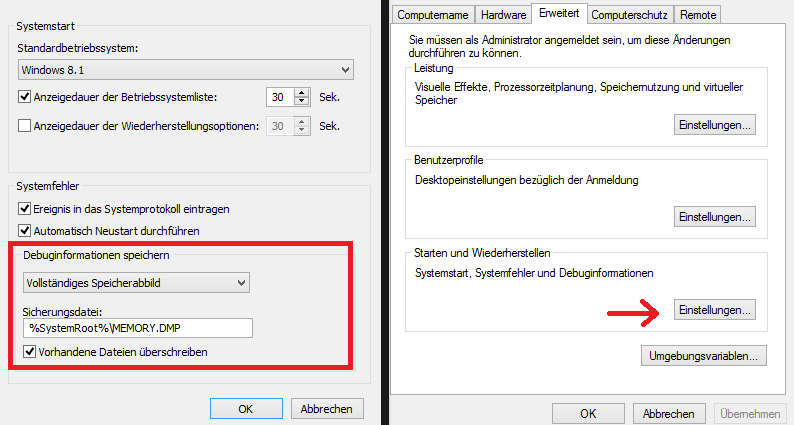
\includegraphics[scale=0.5]{Bilder/RAM.png}
  \caption{Einstellungen für RAM-Seicher Dmp-File}
  \label{ram}
\end{figure}

\noindent Ruft man nun einen STOP-Error herbei, so wird ein gesamtes Speicherabbild im angegeben Pfad gespeichert. Ein solchen Fehler absichtlich auszulösen kann über eine Tastenkombination, die zuvor in einem Registry Eintrag definiert wird, ausgelöst werden. Ein Beispiel dafür wäre:\\\\
\noindent\emph{HKEY\_LM \textbackslash System\textbackslash CurrentControlSet\textbackslash Services\textbackslash i8042prt\textbackslash ParamtersValue \newline Name: CrashOnCtrlScrollData Type: REG\_DWORDData:(1 = enabled)}\\\\
\noindent Nun kann durch das Halten der Strg-Taste und das zweimalige Tippen auf Rollen ein STOP-Error ausgelöst werden. Programme, mit denen man nun das Dmp-File bearbeiten kann werden von Windows selbst bereitgestellt.\\

\noindent\textbf{Speicherabbild des Festplattenspeichers}\\
\noindent Neben ein RAM-Speicherabbild wird bei einer ausführlichen Analyse ein Speicherabbild der Festplatte benötigt. Es gibt spezielle Anwendungen die ein komplettes Speicherabbild der Festplatte erstellen können. Als kommerzielle Lösung stellt Symantec Norton Ghost zur Verfügung. Um eine forensische Analyse durchzuführen werden meist jedoch speziellere Tools verwendet. Eine kostenlose Möglichkeit ein Festplattenabbild zu erstellen ist durch das dd Tool möglich. Dieses ist sowohl für Linux als auch für Windows verfügbar und kopiert Blockweise Speicher von einer Festplatte oder Partition auf einer andere. In Abb. \ref{fest} wird die komplette Partition f: auf d: als cdisk.img gespeichert.\\

\begin{figure}[h]
    \centering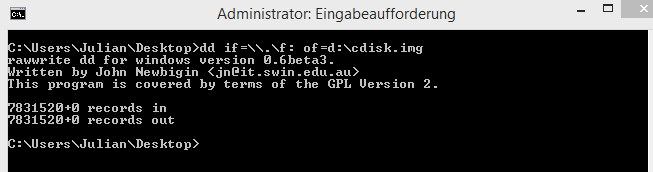
\includegraphics[scale=0.7]{Bilder/DD.png}
  \caption{Erstellung eines Speicherabbilds mit dd}
  \label{dd}
\end{figure}

\noindent Neben dieser vereinfachten Methode gibt es noch weitere Möglichkeiten über kommerzielle Software, die für den Zweck einer forensischen Analyse entwickelt wurden, ein professionelles Festplattenabbild zu erstellen. Zu diesen gehören:
\begin{itemize}
\item EnCase
\item Winhex
\item ProDiscover
\item SafeBack
\end{itemize}

\noindent Nachdem alle relevanten Daten gesichert wurden kann der Netzverkehr überprüft werden.
\subsection{Netzwerkanalyse}
Mit einer Netzwerkanalyse kann am schnellsten erkannt werden, was auf einem Honeypot passiert ist. Die Netzwerkanalyse kann grundsätzlich auf zwei Wege genutzt werden. Zum einem kann erkannt werden welche Ports verwendet wurden, zum anderen kann über die Payload der Pakete nach Details geforscht werden. Wenn der übertragenen Datenverkehr nicht verschlüsselt ist, kann ein Packet-Sniffer (z.B. WireShark) den kompletten Verkehr aufzeichnen. Fragen, die sich bei der Netzwerkanalyse stellen, sind:

\begin{itemize}
\item Wie viele Pakete wurden aufgezeichnet
\item Welche IP Adressen waren beteiligt
\item Wer kommunizierte mit wem
\item Welche Ports wurden verwendet
\item Welche zeitlichen Abstände befinden sich zwischen den abgesendeten Paketen
\item Wie groß waren die Pakete
\end{itemize} 

\noindent Da bei einem länger aktiven Honeypot eine sehr große Menge an Daten in Log-Files gespeichert werden können, sollte sich nicht auf jeden einzelne Kommunikationsvorgang, sondern eher auf die \emph{top talker} (diejenigen, die am meisten kommuniziert haben) geachtet werden. Packet-Sniffer bieten meist die Möglichkeit nach bestimmten Ziel- oder Quell Adressen, Ports oder Protokollen zu filtern. Der zeitliche Abstand verdächtiger Pakete kann Auskunft geben, ob ein Angriff automatisch oder manuell stattfand. Häufig sind Angriffe, die innerhalb von kurzen Zeitintervallen stattfinden, automatisiert. 
Außerdem sollte auf die Paketgröße geachtet werden. Kleine Pakete sind meist Handshake- Broadcast- oder Protocol-overhead Pakete, und können (je nach zu analysierenden Angriff) ignoriert werden. 

Nachdem die Pakete nach den gewünschten Kriterien gefiltert wurden, kann versucht werden ein Muster aus den verschiedenen Paketen zu erkennen.\\

\begin{figure}[h]
    \centering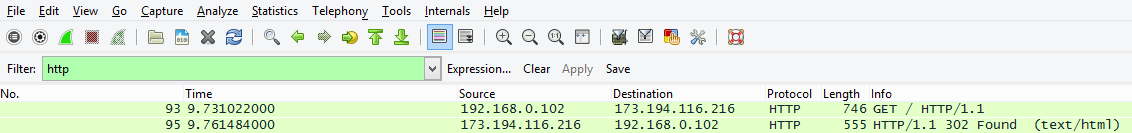
\includegraphics[scale=0.5]{Bilder/Wireshark.png}
  \caption{Packet-Sniffer Wireshark }
  \label{ws}
\end{figure}
\subsection{Analyse des Dateisystems}
Bei der Analyse des Dateisystems kann festgestellt werden welche Dateien hinzugefügt, gelöscht oder verändert wurden. Außerdem kann nach Daten gesucht werden die nicht in Dateien gespeichert wurden (z.B. in unbenutzten Regionen der Festplatte). Eine einfache Methode dies zu bewerkstelligen wäre das Vergleichen des \emph{"zuletzt geändert"} Attribut jedes Ordners bzw. jeder Datei. Programme wie AFind listen alle Daten bezüglich des Veränderungsdatums auf. Dabei ist zu beachten das das System selbst manche Daten ändert und sich das Datum so ebenfalls ändern kann. Diese Methode ist jedoch nur begrenzt effektive, da es allgemein relativ leicht für Hacker möglich ist, die Systemzeit oder ein Zeitstempel einer Datei oder eines Verzeichnisses zu manipulieren. 

Eine effektivere Lösung bietet das \emph{"hashen"} von Dateien. Beim hashen werden große Ursprungsdaten auf eine kleine Datenmenge abgebildet. Ändert sich die eigentliche Datei nur minimal, ändert sich auch der darüber gebildete Hashwert. So kann, wenn man über den ursprüngliche Hashwert verfügt, über einen Vergleich des alten und des neuen Hashwerts überprüfen, ob sich eine Datei verändert hat. 
Über jede Datei des Honeypots sollte vor Produktivschaltung ein Hashwert gebildet werden. Dies kann über verschiedenen kostenfreie Anwendungen stattfinden. Ein Beispiel dafür ist FileCheckMD5. Dieses Scannt rekursiv Verzeichnisse und bildet Hashwerte über die beinhalteten Dateien. Die Werte werden dabei gespeichert und können für die spätere Überprüfung verwendet werden.

\subsection{Analyse des Schadcodes und des Betriebssystems}
Abhängig von der modifizierten Datei oder des modifizierten Systems können nun verschiedene Arten der weiteren Analyse folgen.\\

\noindent\textbf{Analyse von Schadcode}\\
\noindent Bei der Analyse von hinzugekommenen oder modifizierten Dateien können je nach Dateiart verschiedenen Analysemethoden verwendet werden. Bei einer einfachen Textdatei kann mit einer String Analyse begonnen werden. Dabei kann nach im Hacker-Jargon oft vorkommende Begriffe wie "warez" oder "greetz" gesucht werden. Wir ein solches Wort gefunden kann davon ausgegangen werden das es von einem Hacker stammt\cite{grimes.2003a}. Unter Linux mit grep, oder Windows mit der bestehenden Windows-Suche kann eine solche Analyse stattfinden. Es gibt jedoch zusätzlich Tools die eine Suche weiterhin spezifizieren werden kann. Zum Beispiel mit Strings.exe der Sysinternale Suite von Microsoft kann nach ASCII oder Unicode Strings gesucht werden. \\

\noindent Ist die verdächtige Datei ausführbar, wird die Analyse des dazugehörigen Assemblercodes herangezogen. Diese Analyseart ist jedoch sehr aufwendig und sollte nur durchgeführt werden, wenn die genaue Vorgehensweise der Datei von Interesse ist. Die meisten hinterlegten ausführbaren Dateien sind in Script-Sprachen geschrieben und oft vollständig kompiliert. Eine Disassemblierung des Codes kann durch verschiedenen Tools stattfinden (z.B. IDA Pro als kostenfreie oder kostenpflichtige Version), eine Analyse des daraus entstehenden Assemblercodes kann meist nur mit sehr guten Kenntnissen der Assemblersprache stattfinden. Es besteht auch die Möglichkeit die Datei an einen Sicherheitsfirma wie McAffee oder Symantec zu schicken \cite{grimes.2003a}. Diese senden meist innerhalb einer Woche eine Rückmeldung zurück ob die Datei boshaft war, oder nicht.\\  

\noindent\textbf{Analyse des Betriebssystems}\\
Auch ohne eine Datei geändert oder hinzugefügt zu haben, kann der Hacker das System für spätere Angriffe verwundbar gemacht haben. Sie könnten Passwörter entfernt, anfällige Anwendungen geöffnet (Ports), oder andere Anpassungen vorgenommen haben. Es gibt einige Tools die ein komplette Systemkonfiguration für einen späteren Vergleich speichern:

\begin{itemize}
\item Winfingerprint: Winfingerprint scannt IP-Adressen und sammelt spezifische Informationen zu den gefundenen PCs. Damit kann überprüft werden, welche Daten das System nach außen verrät. Der Scanner erkennt das eingesetzte Betriebssystem einschließlich installierter Service Packs, Datei- und Druckerfreigaben, vorhandene Laufwerke, System-ID, Benutzer, Domäne oder Arbeitsgruppe und Dienste (freigeschaltet Ports) des PCs.
\item WinInterrogate: Wininterrogate ist ein Programm für die Anzeige, Überwachung und Katalogisierung von Prozessen. Es listet alle Prozesse und die zugehörigen DLLs auf oder listet alle DLLs auf und ihre Prozesszugehörigkeiten.
\end{itemize}

\noindent Eine Kombination dieser beiden Tools stellt die Grundlage einer Analyse des Betriebssystems dar. Nun kann noch nach weiteren Änderungen gesucht werden:

\begin{itemize}
\item Unter Windows sollten Änderungen in der Registry betrachtet werden (Besonders die Autorun-Schlüssel)
\item Neue auffällige Prozesse sollten genauer untersucht werden
\item Geöffnete Ports und deren zugewiesene Dienste sollten überprüft werden
\end{itemize} 

\noindent Nachdem das Betriebssystem und Dateien nach auffälligen Änderungen durchsucht wurde, ist es an der Zeit die richtigen Schlüsse daraus zu ziehen.
\subsection{Abschließende Schlussfolgerung}
Nachdem die Datenanalyse erfolgreich war, ist festzulegen welche Informationen interessant waren, oder welche bereits bekannt. Meist kann nach folgenden Kriterien ein Angriff klassifiziert werden:

\begin{itemize}
\item Wurde eine andere Angriffsmethode verwendet (im Vergleich zu vorhergehenden Angriffen und Analysen)
\item Welche Verschlüsselung wurde verwendet
\item Wurde ein unübliches Protokoll verwenden
\item War der Angriff auf den Honeypot gerichtet oder war es Zufall
\item Was kann aus dem Angriff gelernt werden
\item Wie kann in Zukunft ein solcher Angriff verhindert werden (falls es sich um einen neuen handelt)
\end{itemize}

\noindent Nach einer Analyse werden üblicherweise Änderungen am Honeypot vorgenommen, um einen wiederholten Angriff dieser Art zu vermeiden. Nachdem alle wichtigen Schlüsse gezogen wurden, muss entschiedene werden wie der Honeypot als nächstes verwendet werden soll. Der Honeypot sollte komplett neu aufgesetzt werden, und kann nun je nach nächsten Verwendungszweck modifiziert werden. Nach einem erneuten Angriff beginnt der Analyseprozess erneut.
